\documentclass{article}
\usepackage{amsmath}
\usepackage{tikz}
\usepackage{graphicx}
\usepackage[toc,page]{appendix}
\usetikzlibrary{positioning}
\begin{document}

\title {consensus high incentive monetary policy}
\author {ertosns}
\date {2023/4/15}
\maketitle


\section{finality control}

\begin{description}
\item The leadership winning mechanism is based off Ouroborous Crypsinous
with some modifications. A stakeholder wins if some random value $y$,
specific to the stakeholder and derived from the blockchain, is less
than target value $T$. The probability of winning is quasi linear with
the relative stake.

\item Accuracy of single leader per slot is affected by percentage of total
DRK tokens in stake, in fact the relation is logarithmic.

\item Assume community $C$ owns 100\% of DRK tokens.

\item The probability of $C$ winning the lottery at any slot is defined as:
  $$P(C=lead) = y < 1 -(1-f)^\alpha $$
  $$= y < 1 -(1-f) $$
  $$= y < f$$

\item In our case f is targetting single leader per slot. An emulation of
the leader election mechanism with PID controllers shows that f is
oscillating around ~0.65 (depending on ration of tokens in stake). then P(C=lead)~=0.65


\item Given the linear independence property of the target function T, the
probability of a node winning leadership at any slot with S staked tokens
is the same as the probability of N nodes winning leadership at same slot,
with same stake S for any S, N values.

\item If the probability of stakeholder owning 10\% of the tokens is 0.035,
then the probability of a pool consisting of stakeholders owning 10%
of tokens is also 0.035.

\item The probability of a pool of N\% stake to win the leadership at any slot is: $$ \frac{N}{100}*P(C=lead)$$



  %\write18{wget http://www.some-site.com/path/to/image.png}
  \begin{figure}[!h]
    \caption {relation of DRK staked vs accuracy of finality}
    \centering
    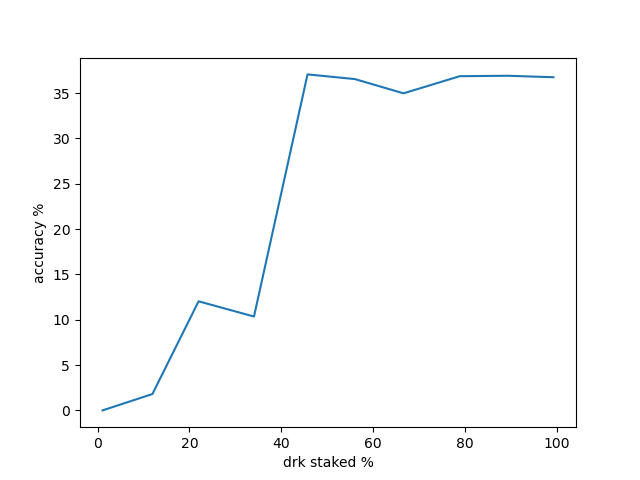
\includegraphics{hodler_acc_vs_sr.png}
    \label{fig:relation of DRK staked vs accuracy of finality}
    \end{figure}


\item Assume $P(C=lead)=33\%$, then if only 10\% of the total network token
is staked the probability of having a single leader per slot is $\frac{10}{100}P(C=lead)=0.035, or accuracy of 3\%.


\item From the graph above, and as a consequence of the linear independence
property the accuracy of the controller leaks the percentage of token
in stake.

\end{description}

\section{cascade control with staked ratio as set point}
\begin{description}
\item to incentivize stakeholders to increase staked token, another reward controller is placed between reward and staked ratio, to incentivize staked ratio to maintain stable single lead accuracy with relatively lower staked ratio.

\end{description}

\begin{figure}
 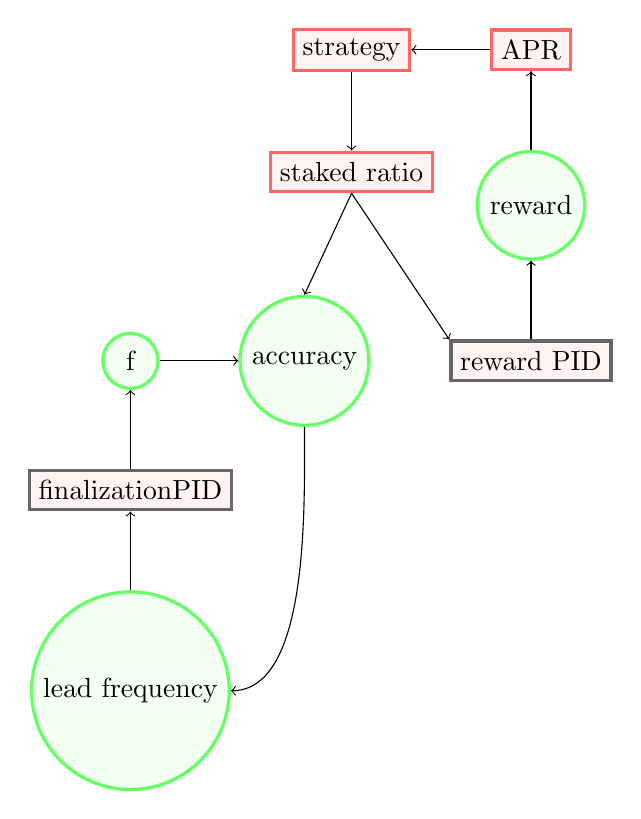
\begin{tikzpicture}[
    roundnode/.style={circle, draw=green!60, fill=green!5, very thick, minimum size=7mm},
    squarednode/.style={rectangle, draw=red!60, fill=red!5, very thick, minimum size=5mm},
    pidnode/.style={rectangle, draw=black!60, fill=red!5, very thick, minimum size=5mm}
   ]
   \node[roundnode]    (f)                                           {f};
   \node[roundnode]  (accuracy)         [right=of f]                {accuracy};
   \node[pidnode]  (finalizationPID)  [below=of f]               {finalizationPID};
   \node[roundnode]  (leadfrequency)    [below=of finalizationPID] {lead frequency};
   \node[pidnode] (rewardPID) [right=of accuracy]  {reward PID};
   \node[roundnode] (reward) [above=of rewardPID] {reward};
   \node[squarednode] (APR) [above=of reward] {APR};
   \node[squarednode] (strategy) [left=of APR] {strategy};
   \node[squarednode] (stakedratio) [below=of strategy] {staked ratio};

  \draw[->] (finalizationPID.north) -- (f.south);
  \draw[->] (f.east) -- (accuracy.west);
  \draw[->] (leadfrequency.north) -- (finalizationPID.south);
  \draw[->] (accuracy.south) .. controls +(down:10mm) and +(right:10mm) .. (leadfrequency.east);
  \draw[->] (stakedratio.south) -- (rewardPID.north west);
  %\draw[->] (accuracy.east) -- (rewardPID.west);
  \draw[->] (rewardPID.north) -- (reward.south);
  \draw[->] (reward.north) -- (APR.south);
  \draw[->] (APR.west) -- (strategy.east);
  \draw[->] (strategy.south) -- (stakedratio.north);
  \draw[->] (stakedratio.south) -- (accuracy.north);
 \end{tikzpicture}
 \caption{cascade PID diagram}
\end{figure}

\begin{description}
\item the finality lead controller works at higher frequency on the slot level, outputs new f value per slot.

\item reward controller works at lower frequency on the epoch level, outputs new reward value per epoch, so reward is static per epoch.
\end{description}
\section{experiments}
\begin{description}
  \subsection{simulation parameters}
  \item finality controller parameters  $kp=-0.0104$, $ki=-0.0366$, $kd=0.0384$, while reward controller parameters  $kp=0.13$, $ki=-0.5$, $kd=-0.5$ on 1000 nodes, running time is 10,000 slots. stakeholders starategy is distributed equally between HODLER: stake it all, linear: stake DRK with ratio equivalent to the APR, logarithmic and sigmoid strategy that have logarithmic, and segmoid relation respectively to APR.

\item when staked ratio is high (100\% in this experiment) reward reduces to 1.33, as a consequence APR 0.2\%, and staked ratio goes down on following epoch.
  \begin{figure}
    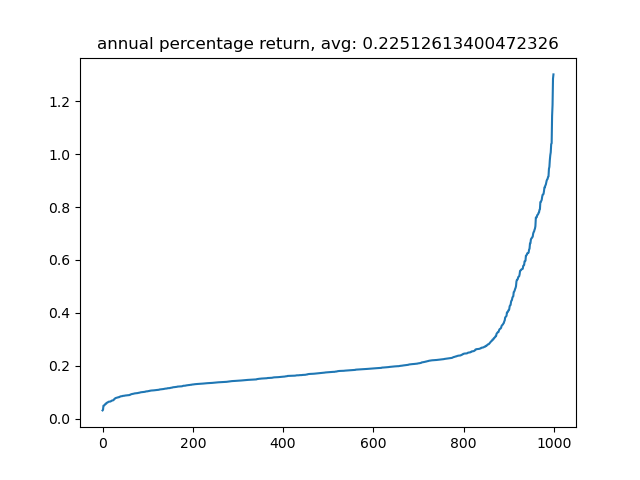
\includegraphics{fullstake_apr.png}
    \caption{apr sorted from left to right in range [0-1.2]\% and 0.2\% on average with 100\% staked ratio}
  \end{figure}
\item while with 68\% staked ratio reward goes up to 82.5 on average with 13.8\% apr and same accuracy as previous experiment 35.7\%
  \begin{figure}
    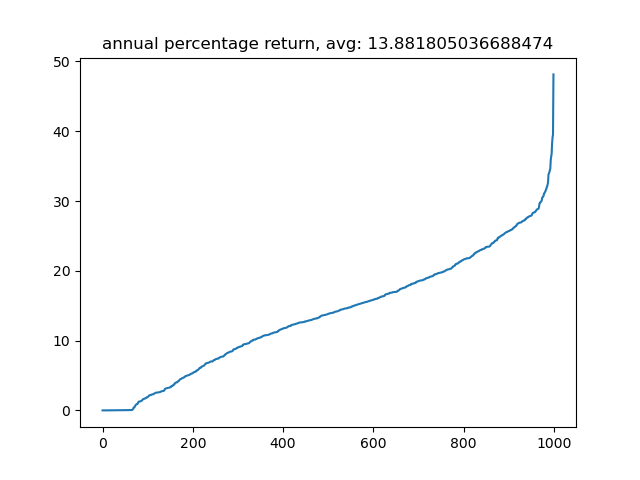
\includegraphics{halfstake_apr.png}
    \caption{apr sorted from left to right in range [1-50]\% and 13.8\% avg apr.}
  \end{figure}

  \subsection {oracle for staked ratio discovery}
  an oracle would be required to figure out the accuracy vs staked ratio curve every epoch.

\end{description}

\section {cascade control with accuracy set point}

\begin{description}
  \item use accuracy as set point for reward PID controller, accuracy being output (although indirect) of the secondary controller at higher frequency plugged as input to the primary reward controller would result in much better accuracy at lower staked ratio, but with lower APR.
\end{description}

\begin{figure}
 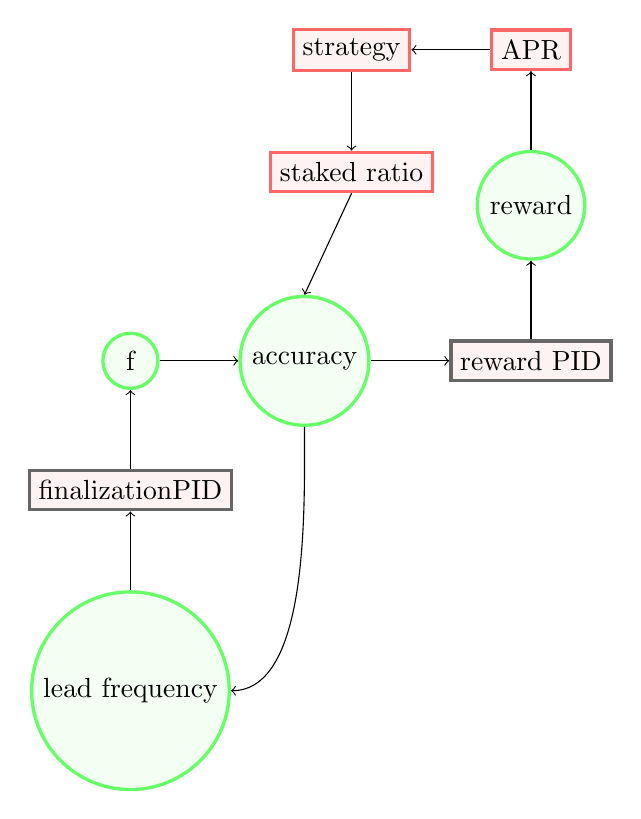
\begin{tikzpicture}[
    roundnode/.style={circle, draw=green!60, fill=green!5, very thick, minimum size=7mm},
    squarednode/.style={rectangle, draw=red!60, fill=red!5, very thick, minimum size=5mm},
    pidnode/.style={rectangle, draw=black!60, fill=red!5, very thick, minimum size=5mm}
   ]
   \node[roundnode]    (f)                                           {f};
   \node[roundnode]  (accuracy)         [right=of f]                {accuracy};
   \node[pidnode]  (finalizationPID)  [below=of f]               {finalizationPID};
   \node[roundnode]  (leadfrequency)    [below=of finalizationPID] {lead frequency};
   \node[pidnode] (rewardPID) [right=of accuracy]  {reward PID};
   \node[roundnode] (reward) [above=of rewardPID] {reward};
   \node[squarednode] (APR) [above=of reward] {APR};
   \node[squarednode] (strategy) [left=of APR] {strategy};
   \node[squarednode] (stakedratio) [below=of strategy] {staked ratio};

  \draw[->] (finalizationPID.north) -- (f.south);
  \draw[->] (f.east) -- (accuracy.west);
  \draw[->] (leadfrequency.north) -- (finalizationPID.south);
  \draw[->] (accuracy.south) .. controls +(down:10mm) and +(right:10mm) .. (leadfrequency.east);
  %\draw[->] (stakedratio.south) -- (rewardPID.north west);
  \draw[->] (accuracy.east) -- (rewardPID.west);
  \draw[->] (rewardPID.north) -- (reward.south);
  \draw[->] (reward.north) -- (APR.south);
  \draw[->] (APR.west) -- (strategy.east);
  \draw[->] (strategy.south) -- (stakedratio.north);
  \draw[->] (stakedratio.south) -- (accuracy.north);
 \end{tikzpicture}
 \caption{cascade PID diagram}
\end{figure}

\subsection {experiments}
\begin{description}
\subsection {simulation parameters}
\item finality controller parameters  $kp=-0.0104$, $ki=-0.0366$, $kd=0.0384$, while reward controller parameters  $kp=-2.53$, $ki=29.5$, $kd=53.77$ on 100 nodes, running time is 10,000 slots.
  \item stakeholders starategy is distributed equally between HODLER: stake it all,  logarithmic and sigmoid strategy that have logarithmic, and segmoid relation respectively to APR. similar to previous experiment except there is no linear strategy since APR is much lower.


\item from figure 1, 25\% staked DRK ratio result in approximately 11\% secondary controller accuracy, while with cascade control it gains 3X leverage at lower staked ratio. 10\% staked ratio results in 30\% accuracy with average reward 1.6 DRK, and 0.2\% APR (see figure 6)
\end{description}
\begin{figure}
    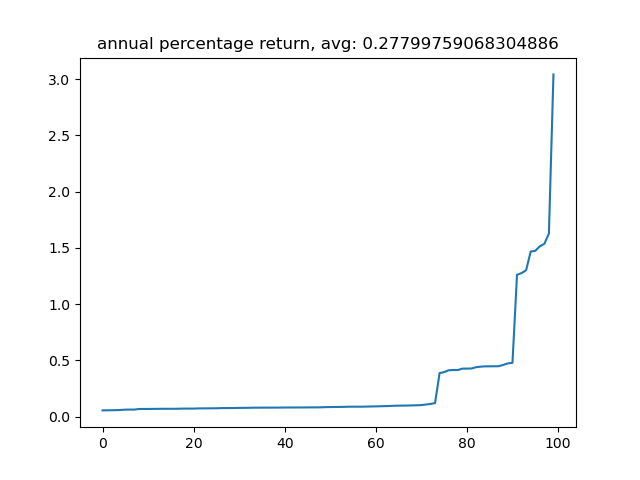
\includegraphics{acc_setpoint_quarterstake.png}
    \caption{with accuracy set point to primary controller}
\end{figure}

\begin{description}
\item figure 7 shows the relation between staked DRK tokens ratio, and accuracy
\end{description}
\begin{figure}
  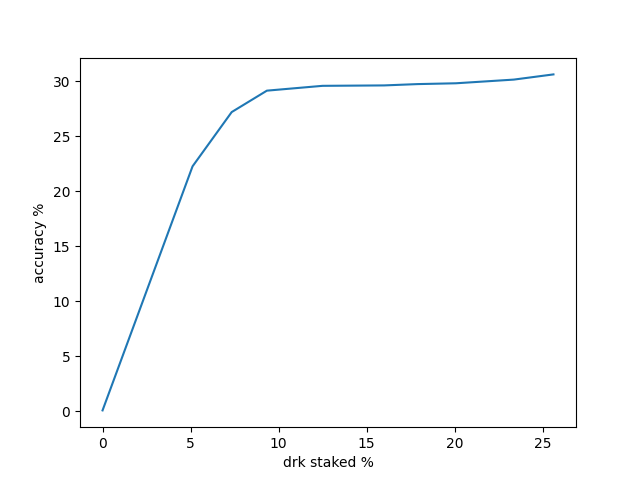
\includegraphics{acc_stake_1000nodes_10kslots_with_cascade.png}
  \caption{relation between staked DRK ratio and accuracy of secondary controller, with accuracy as set point to primary controller}
\end{figure}


\section{conclusion}
cascade control with accuracy as set point is leveraging accuracy of secondary controller of single leader per slot at low APR, while staked DRK ratio as set point can be highly inflationary, with high APR, and relatively enhanced accuracy at lower staked ratio. the former is much simpler, doesn't require staked ratio curve oracle.

\end{document}
